\documentclass[11pt]{article}
\usepackage{psfig}
\usepackage{latexsym}
\usepackage{amsfonts}
\usepackage{amsmath}
\usepackage{tikz}
\usetikzlibrary{circuits.logic.US}
\setlength{\textheight}{8.5in}
\setlength{\textwidth}{6.0in}
\setlength{\headheight}{0in}
\addtolength{\topmargin}{-.5in}
\addtolength{\oddsidemargin}{-.5in}
\usepackage{array}

\input{hw-preamble.tex}
\begin{document}


%\lecture{1}{October 29, 2019}{Adi Akavia}{(your name here)}
\hw{1}{Fall 2021}{Dr. Adi Akavia}{(Aya)}
%%%% body goes in here %%%%

\section*{problem 1}
Truth table:
\begin{center}
\begin{tabular}{ | m{1cm} | m{.5cm} | m{.5cm} | m{.5cm}| m{.5cm} | } 
  \hline
  $\alpha$ \textbackslash x  & 0 & 1 & 2 & 3 \\ 
  \hline
  0 & 0 & 0 & 0 & 0 \\ 
  \hline
  1 & 0 & 0 & 0 & 0\\ 
  \hline
  2 & 0 & 0 & 1 & 1 \\ 
  \hline
  3 & 0 & 0 & 1 & 1\\ 
  \hline
\end{tabular}
\end{center}


 DNF of truth table for equation (2) when every variable is presented as binary value:
 
 \begin{equation*}
 (\lnot a_1\wedge a_0\wedge\lnot x_1\wedge x_0)\cup(a_1\wedge a_0\wedge\lnot x_1\wedge x_0)\cup(\lnot a_1\wedge a_0\wedge x_1\wedge x_0)\cup(a_1\wedge a_0\wedge x_1\wedge x_0)=\end{equation*} 
 \begin{equation*}
 ((\lnot a_0\cup a_0)\wedge a_1 \wedge{ \lnot x}_0 \wedge x_1)\cup(( \lnot a_0 \cup a_0)\wedge a_1\wedge x_0\wedge x_1)=\end{equation*}  \begin{equation*}(a_1\wedge{\lnot x}_0\wedge x_1)\cup(a_1\wedge x_0\wedge x_1)=(a_1\wedge{(\lnot x}_0\cup x_0)\wedge x_1)=(a_1\wedge x_1)
 \end{equation*}
   

\section*{problem 2}


 \begin{equation*} \overrightarrow{a} = (a_{1}, a_{2})\end{equation*}   \begin{equation*}
    \overrightarrow{x} = (x_{1}, x_{2})
\end{equation*}  \begin{equation*}\overrightarrow{a},\overrightarrow{x} \in{0,1,2,3^2}  \end{equation*}
where each entry is specified in binary representation. Namely:   \begin{equation*}
a_1=(a_{11},a_{10})\in{{{0,1}}}^2,a_2=(a_{21},a_{20})\in{{0,1}}^2,x_1=(x_{11},x_{10})\in{{0,1}}^2,x_2=(x_{21},x_{20})\in{{0,1}}^2
\end{equation*}
We will divide into cases and add OR gate between them:

\underline{Case 1:}
\begin{equation}  a_1 x_1 \geq 4 \cup a_2 x_2 \geq 4\end{equation} and we'll use the DNF we found before for equation (2):
\begin{table}[ht!]
\centering
\begin{tabular}{ | m{1cm} | m{.8cm} | m{.8cm} | m{.8cm}| m{.8cm} | } 
  \hline
  $\alpha$ \textbackslash  x & 00 & 01 & 10 & 11 \\ [1 ex] 
 \hline\hline
 00 & 0 & 0 & 0 & 0\\ 
01 & 0 & 0 & 0 & 0\\
 10 & 0 & 0 & 1 & 1 \\
 11 & 0 & 0 & 1 & 1\\ [1ex] 
 \hline
\end{tabular}
\label{table2:data}
\end{table}
\begin{equation*}
(a_{11} \wedge x_{11} \cup a_{21} \wedge x_{21})
\end{equation*}
 %%\includegraphics{BooleanCircuit1.PNG}
 We use the fact that:
 \begin{equation*}
     A\cup B=(A\oplus B) \oplus (A\wedge B)
 \end{equation*}
 Then:
 \begin{equation*}
   ((a_{11} \wedge x_{11} )\cup (a_{21} \wedge x_{21}))= \end{equation*}  \begin{equation*}
        ((a_{11} \wedge x_{11})\oplus(a_{21} \wedge x_{21}))\oplus ((a_{11} \wedge x_{11} )\wedge (a_{21} \wedge x_{21}))=
    \end{equation*} \begin{equation*}
        ((a_{11} \wedge x_{11})\oplus(a_{21} \wedge x_{21}))\oplus (a_{11} \wedge x_{11} \wedge a_{21} \cup x_{21})
    \end{equation*}
     \underline{Case 2:}
\begin{equation}  a_1 x_1 \geq 2 \cap a_2 x_2 \geq 2\end{equation}
\begin{table}[ht!]
\centering
\begin{tabular}{ | m{1cm} | m{.8cm} | m{.8cm} | m{.8cm}| m{.8cm} | } 
  \hline
  $\alpha$ \textbackslash  x & 00 & 01 & 10 & 11 \\ [1 ex] 
 \hline\hline
 00 & 0 & 0 & 0 & 0\\ 
01 & 0 & 0 & 1 & 1\\
10 & 0 & 1 & 1 & 1 \\
11 & 0 & 1 & 1 & 1\\ [1ex] 
 \hline
\end{tabular}
\end{table}

for Implement that case we've used DNF and got that:

\begin{equation*}
((a_{10} \cap x_{11}) \cup (a_{11} \cap x_{10})) \cap ((a_{20} \cap x_{21}) \cup (a_{21} \cap x_{20})) 
\end{equation*}

 We use the fact that:
 
 \begin{equation*}
     A\cup B=(A\oplus B) \oplus (A\wedge B)
 \end{equation*}
 
 \begin{equation*}
 ((a_{10}\cap x_{11})\cup (a_{11}\cap x_{10})) \cap ((a_{20}\cap x_{21})\cup (a_{21}\cap x_{20}))= \end{equation*}
 

      $((((a_{10}\cap x_{11})\oplus (a_{11}\cap x_{10})) \oplus  ((a_{10}\cap x_{11})\wedge (a_{11}\cap x_{10})))\cap((((a_{20}\cap x_{21})\oplus (a_{21}\cap x_{20}))\oplus ((a_{20}\cap x_{21})\wedge (a_{21}\cap x_{20}))) $
      
      
 \underline{Case 3:}
 \begin{equation} ( a_1 x_1 \geq 3 \cap a_2 x_2 \geq 1)  \end{equation}
Truth table for :$ ax\geq 3 $  

\begin{table}[ht!]
\centering
\begin{tabular}{ | m{1cm} | m{.8cm} | m{.8cm} | m{.8cm}| m{.8cm} | } 
  \hline
  $\alpha$ \textbackslash  x & 00 & 01 & 10 & 11 \\ [1 ex] 
 \hline\hline
 00 & 0 & 0 & 0 & 0\\ 
 01 & 0 & 0 & 1 & 0\\
 10 & 0 & 1 & 1 & 1 \\
 11 & 0 & 0 & 1 & 1\\ [1ex] 
 \hline
\end{tabular}
\end{table}
Truth table for :$ ax\geq 1 $ 
\begin{table}[ht!]
\centering
\begin{tabular}{ | m{1cm} | m{.8cm} | m{.8cm} | m{.8cm}| m{.8cm} | } 
  \hline
  $\alpha$ \textbackslash  x & 00 & 01 & 10 & 11 \\ [1 ex] 
 \hline\hline
00 & 0 & 0 & 0 & 0\\ 
01 & 0 & 1 & 1 & 1\\
10 & 0 & 1 & 1 & 1 \\
11 & 0 & 1 & 1 & 1\\ [1ex] 
 \hline
\end{tabular}
\end{table}

 for Implement that case we've used DNF and got that for $( a_1 x_1 \geq 3 \cap a_2 x_2 \geq 1)$
  \begin{equation*}
      ((a_{11} \cap x_{11})\cup (x_{11}\cap a_{10} \cap x_{10})\cup (a_{10}\cap a_{11} \cap x_{10}))\cap ((x_{21}\cap a_{20}) \cup (x_{20}\cap a_{20})\cup(x_{21}\cap a_{21}))\cup (x_{20}\cap a_{21})
  \end{equation*}
\underline{Case 4:}
 \begin{equation} ( a_1 x_1 \geq 1 \cap a_2 x_2 \geq 3)  \end{equation}  
  for Implement that case we've used DNF and got that for $( a_1 x_1 \geq 1 \cap a_2 x_2 \geq 3)$
  \begin{equation*}
      ((a_{21} \cap x_{21})\cup (x_{21}\cap a_{20} \cap x_{20})\cup (a_{20}\cap a_{21} \cap x_{20}))\cap ((x_{11}\cap a_{10}) \cup (x_{10}\cap a_{10})\cup(x_{11}\cap a_{11}))\cup (x_{10}\cap a_{11})
  \end{equation*}
We do the same in case 3 to replace the OR and put XOR instead and then we put OR between case 1 case 2 case 3 case 4 and do the same to get XOR instead of OR.
\subsection*{The boolean circuit:}

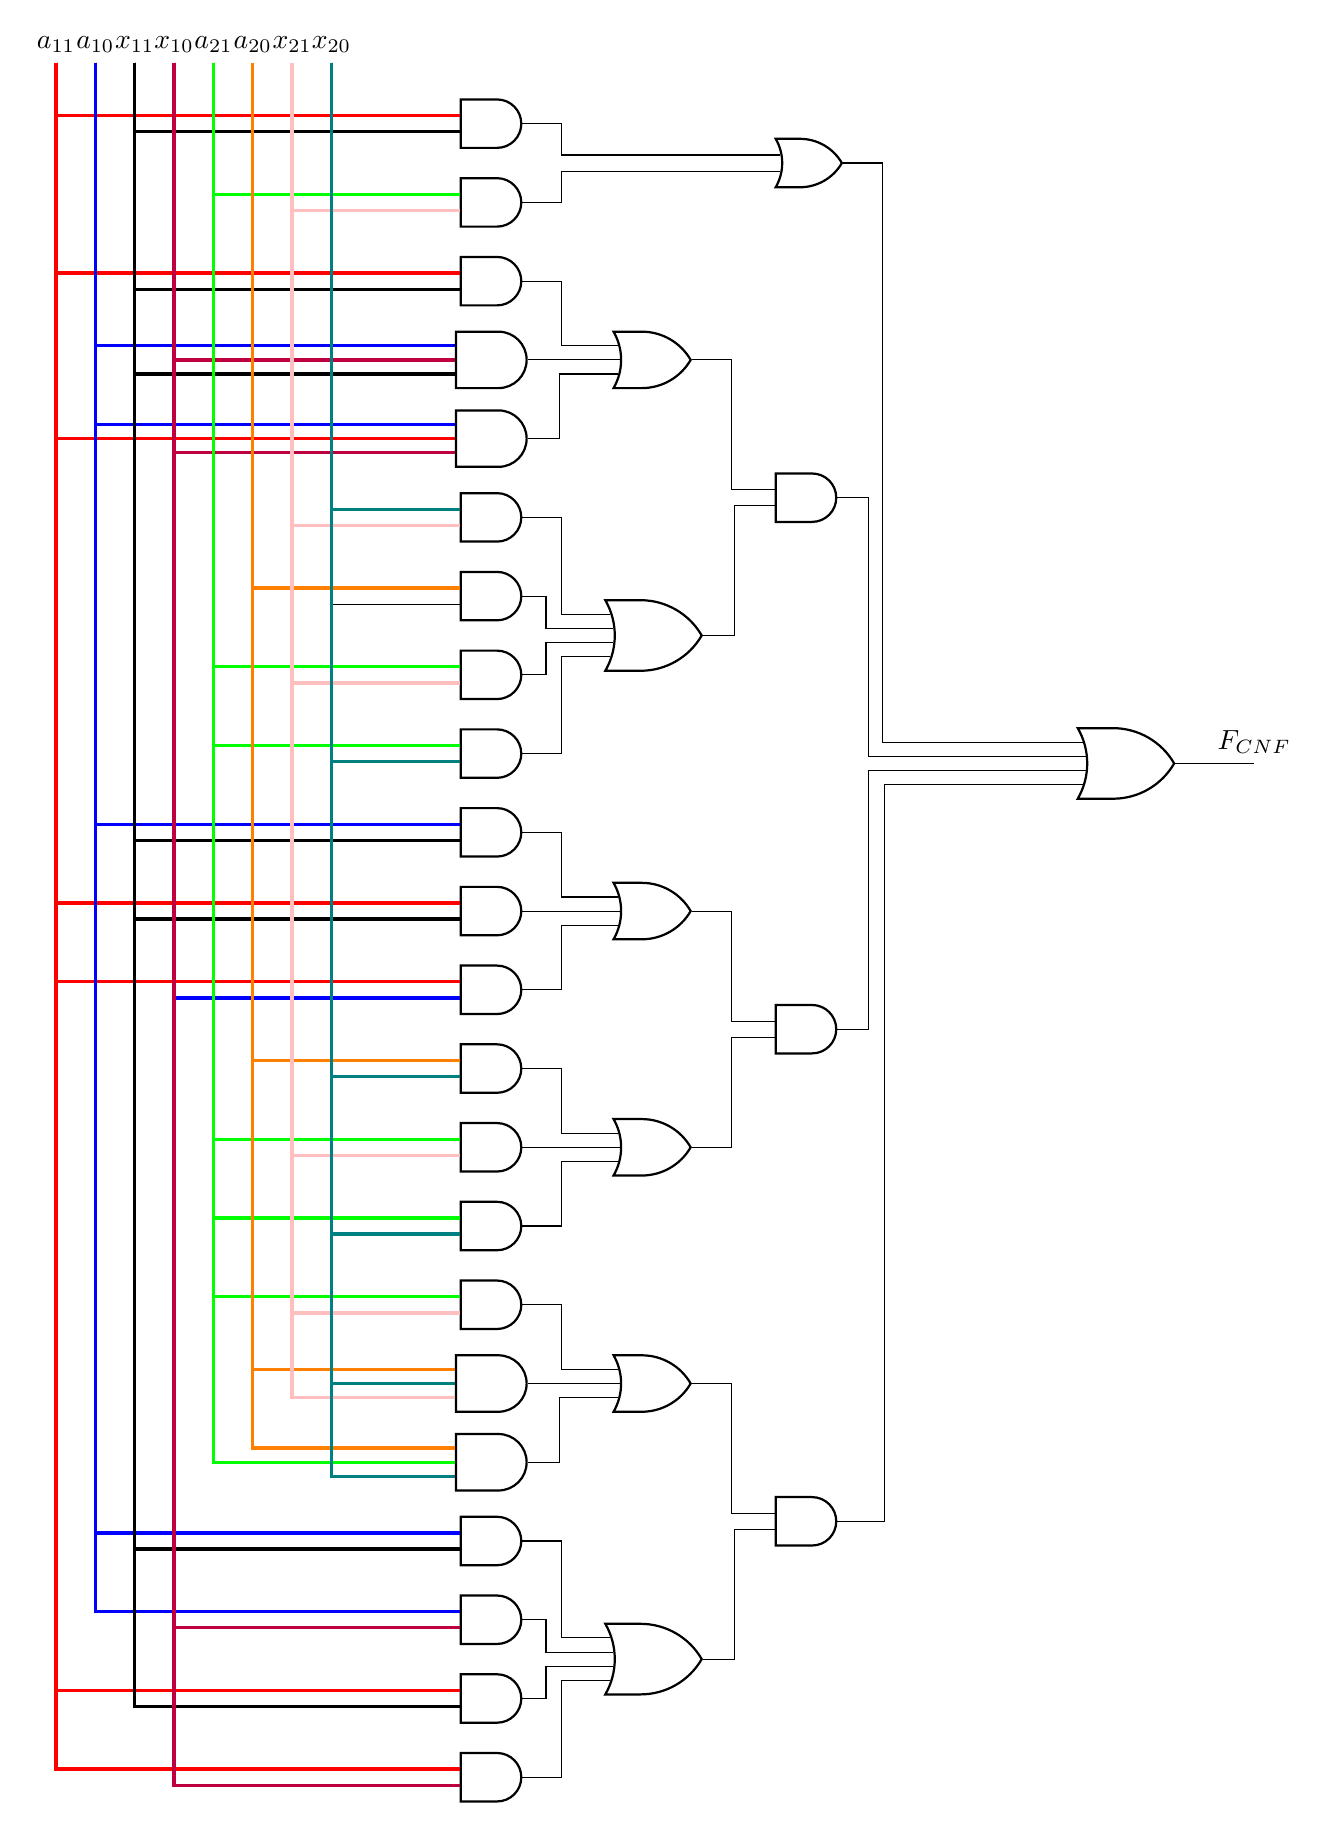
\begin{tikzpicture}[circuit logic US, every circuit symbol/.style={thick}]

\node (a11) at (-7.5,6) {$a_{11}$};
\node (a10) at (-7,6) {$a_{10}$};
\node (x11) at (-6.5,6) {$x_{11}$};
\node (x10) at (-6,6) {$x_{10}$};

\node (a21) at (-5.5,6) {$a_{21}$};
\node (a20) at (-5,6) {$a_{20}$};
\node (x21) at (-4.5,6) {$x_{21}$};
\node (x20) at (-4,6) {$x_{20}$};


\node[and gate,inputs={nn}, point right] (and1) at (-2,5)    {};
\node[and gate,inputs={nn}, point right] (and2) at (-2,4)    {};

\node[and gate,inputs={nn}, point right] (and3) at (-2,3)    {};
\node[and gate,inputs={nnn}, point right] (and4) at (-2,2)    {};
\node[and gate,inputs={nnn}, point right] (and5) at (-2,1)    {};

\node[and gate,inputs={nn}, point right] (and6) at (-2,0)    {};
\node[and gate,inputs={nn}, point right] (and7) at (-2,-1)    {};
\node[and gate,inputs={nn}, point right] (and8) at (-2,-2)    {};
\node[and gate,inputs={nn}, point right] (and9) at (-2,-3)    {};

\node[and gate,inputs={nn}, point right] (and10) at (-2,-4)    {};
\node[and gate,inputs={nn}, point right] (and11) at (-2,-5)    {};
\node[and gate,inputs={nn}, point right] (and12) at (-2,-6)    {};

\node[and gate,inputs={nn}, point right] (and13) at (-2,-7)    {};
\node[and gate,inputs={nn}, point right] (and14) at (-2,-8)    {};
\node[and gate,inputs={nn}, point right] (and15) at (-2,-9)    {};

\node[and gate,inputs={nn}, point right] (and16) at (-2,-10)    {};
\node[and gate,inputs={nnn}, point right] (and17) at (-2,-11)    {};
\node[and gate,inputs={nnn}, point right] (and18) at (-2,-12)    {};

\node[and gate,inputs={nn}, point right] (and19) at (-2,-13)    {};
\node[and gate,inputs={nn}, point right] (and20) at (-2,-14)    {};
\node[and gate,inputs={nn}, point right] (and21) at (-2,-15)    {};
\node[and gate,inputs={nn}, point right] (and22) at (-2,-16)    {};

\node[or gate,inputs={nn}, point right] (or1) at (2,4.5)    {};
\node[or gate,inputs={nnn}, point right] (or2) at (0,2)    {};
\node[or gate,inputs={nnnn}, point right] (or3) at (0,-1.5)    {};
\node[or gate,inputs={nnn}, point right] (or4) at (0,-5)    {};
\node[or gate,inputs={nnn}, point right] (or5) at (0,-8)    {};
\node[or gate,inputs={nnn}, point right] (or6) at (0,-11)    {};
\node[or gate,inputs={nnnn}, point right] (or7) at (0,-14.5)    {};

\node[and gate,inputs={nn}, point right] (and23) at (2,0.25)    {};
\node[and gate,inputs={nn}, point right] (and24) at (2,-6.5)    {};
\node[and gate,inputs={nn}, point right] (and25) at (2,-12.75)    {};

\node[or gate,inputs={nnnn}, point right] (or8) at (6,-3.125)    {};

\draw (and23.output) -- ([xshift=0.4cm]and23.output) |- (or8.input 2);
\draw (or1.output) -- ([xshift=0.5cm]or1.output) |- (or8.input 1);
\draw (and24.output) -- ([xshift=0.4cm]and24.output) |- (or8.input 3);
\draw (and25.output) -- ([xshift=0.6cm]and25.output) |- (or8.input 4);

\draw (or2.output) -- ([xshift=0.5cm]or2.output) |- (and23.input 1);
\draw (or3.output) -- ([xshift=0.4cm]or3.output) |- (and23.input 2);

\draw (or4.output) -- ([xshift=0.5cm]or4.output) |- (and24.input 1);
\draw (or5.output) -- ([xshift=0.5cm]or5.output) |- (and24.input 2);

\draw (or6.output) -- ([xshift=0.5cm]or6.output) |- (and25.input 1);
\draw (or7.output) -- ([xshift=0.4cm]or7.output) |- (and25.input 2);

\draw (and1.output) -- ([xshift=0.5cm]and1.output) |- (or1.input 1);
\draw (and2.output) -- ([xshift=0.5cm]and2.output) |- (or1.input 2);

\draw (and3.output) -- ([xshift=0.5cm]and3.output) |- (or2.input 1);
\draw (and4.output) -- ([xshift=0.5cm]and4.output) |- (or2.input 2);
\draw (and5.output) -- ([xshift=0.4cm]and5.output) |- (or2.input 3);

\draw (and6.output) -- ([xshift=0.5cm]and6.output) |- (or3.input 1);
\draw (and7.output) -- ([xshift=0.3cm]and7.output) |- (or3.input 2);
\draw (and8.output) -- ([xshift=0.3cm]and8.output) |- (or3.input 3);
\draw (and9.output) -- ([xshift=0.5cm]and9.output) |- (or3.input 4);

\draw (and10.output) -- ([xshift=0.5cm]and10.output) |- (or4.input 1);
\draw (and11.output) -- ([xshift=0.5cm]and11.output) |- (or4.input 2);
\draw (and12.output) -- ([xshift=0.5cm]and12.output) |- (or4.input 3);

\draw (and13.output) -- ([xshift=0.5cm]and13.output) |- (or5.input 1);
\draw (and14.output) -- ([xshift=0.5cm]and14.output) |- (or5.input 2);
\draw (and15.output) -- ([xshift=0.5cm]and15.output) |- (or5.input 3);

\draw (and16.output) -- ([xshift=0.5cm]and16.output) |- (or6.input 1);
\draw (and17.output) -- ([xshift=0.5cm]and17.output) |- (or6.input 2);
\draw (and18.output) -- ([xshift=0.4cm]and18.output) |- (or6.input 3);

\draw (and19.output) -- ([xshift=0.5cm]and19.output) |- (or7.input 1);
\draw (and20.output) -- ([xshift=0.3cm]and20.output) |- (or7.input 2);
\draw (and21.output) -- ([xshift=0.3cm]and21.output) |- (or7.input 3);
\draw (and22.output) -- ([xshift=0.5cm]and22.output) |- (or7.input 4);

\draw [red, very thick] (a11) |- (and1.input 1);
\draw [black, very thick] (x11) |- (and1.input 2);

\draw [green, very thick]  (a21) |- (and2.input 1);
\draw [pink, very thick] (x21) |- (and2.input 2);

\draw [red, very thick] (a11) |- (and3.input 1);
\draw [black, very thick] (x11) |- (and3.input 2);

\draw [blue, very thick] (a10) |- (and4.input 1);
\draw [purple , very thick] (x10) |- (and4.input 2);
\draw [black, very thick] (x11) |- (and4.input 3);

\draw [blue, very thick] (a10) |- (and5.input 1);
\draw [red, very thick] (a11) |- (and5.input 2);
\draw [purple , very thick] (x10) |- (and5.input 3);

\draw [teal , very thick] (x20) |- (and6.input 1);
\draw [pink, very thick] (x21) |- (and6.input 2);

\draw [orange, very thick] (a20) |- (and7.input 1);
\draw (x20) |- (and7.input 2);

\draw  [green, very thick] (a21) |- (and8.input 1);
\draw [pink, very thick] (x21) |- (and8.input 2);

\draw [green, very thick] (a21) (a21) |- (and9.input 1);
\draw [teal , very thick] (x20) |- (and9.input 2);

\draw [blue, very thick] (a10) |- (and10.input 1);
\draw [black, very thick] (x11) |- (and10.input 2);

\draw [red, very thick] (a11) |- (and11.input 1);
\draw [black, very thick] (x11) |- (and11.input 2);

\draw [red, very thick] (a11) |- (and12.input 1);
\draw [blue, very thick] (x10) |- (and12.input 2);

\draw [orange, very thick] (a20) |- (and13.input 1);
\draw [teal , very thick] (x20) |- (and13.input 2);

\draw [green, very thick] (a21) (a21) |- (and14.input 1);
\draw [pink, very thick] (x21) |- (and14.input 2);

\draw [green, very thick] (a21) (a21) |- (and15.input 1);
\draw [teal , very thick] (x20) |- (and15.input 2);

\draw [green, very thick] (a21) (a21) |- (and16.input 1);
\draw [pink, very thick] (x21) |- (and16.input 2);

\draw [orange, very thick] (a20) |- (and17.input 1);
\draw [teal , very thick] (x20) |- (and17.input 2);
\draw [pink, very thick] (x21) |- (and17.input 3);

\draw [orange, very thick] (a20) |- (and18.input 1);
\draw [green, very thick] (a21) (a21) |- (and18.input 2);
\draw [teal , very thick] (x20) |- (and18.input 3);

\draw [blue, very thick] (a10) |- (and19.input 1);
\draw [black, very thick] (x11) |- (and19.input 2);

\draw [blue, very thick] (a10) |- (and20.input 1);
\draw [purple , very thick] (x10) |- (and20.input 2);

\draw [red, very thick] (a11) |- (and21.input 1);
\draw [black, very thick] (x11) |- (and21.input 2);

\draw [red, very thick] (a11) |- (and22.input 1);
\draw [purple , very thick] (x10) |- (and22.input 2);

\draw (or8.output) -- ++(right:10mm) node [above]{$F_{CNF}$};

\end{tikzpicture}
\section*{problem 3}
We first create a help circuit $G_{4} : GF(11) \to GF(11)$ such that $G_{4}(a) = 0 \Leftrightarrow 0\leq a < 4$ this can be easily done with  \[G(x) = \left(x\cdot(x-1)\right) \cdot \left((x-2)\cdot(x-3)\right)\].
we will use the following fact, for every two numbers a,b such $a+b \geq 4$ then $G_{4}(a) \vee G_{4}(b) \vee G_{4}(a+b mod 11) = True$ (when considering 0 as false and true otherwise). We also notate the operation $B(a) = a^{10}$ (computed with 4 multiplications) 
Now we can easily construct a circuit 
\[c_0 = \alpha_0\cdot x_0, c_1 = \alpha_1\cdot x_1\]
\[B((B(G(c_0))+B(G(c_1)))+B(G(c_0+c_1)))\] when applying B on the sum acts as applying or on the outputs.

\section*{problem 4}

% \subsection{analysing problem 2}
% 

% for understanding the depth we will first understand the depth of summation. 
% \[depth(O_0) = 1+max\{depth(x_0),depth(y_0)\}\]
% \[depth_{\times}(O_0) = max\{depth(x_0),depth(y_0)\}\]
% \[depth(O_1) = max{1+max\{depth(x_0),depth(y_0)\}}\]
\subsection{analysing problem 2}
We can analyze circuit depth acording to the boolean circuit we draw before every OR gate is equal to 3 since $  A\cup B=(A\oplus B) \oplus (A\wedge B)$ so according to our boolean circuit circuit depth=8, So on in calculating the size every OR gate is equal to 3,so circuit $size=49$, MULT is equal to number of multiplication operations we can look in the circuit we draw and every OR is equal to one multiplication operation since we can change it to XOR by using this $  A\cup  B=(A\oplus B) \oplus (A\wedge B)$ so in this case $MULT=33$,and the multiplicative depth (x-depth) that captures
the maximal distance between an input and an output when counting only multiplication, considering OR as 1 multiplication x-depth=4
\subsection{analysing problem 3}
The depth is $depth(B)+2+depth(B)+depth(G)+1$, the or operation taking $depth(B)+2+depth(B)$ while the separate $G$ testing takes another $depth(G)$ plus one for the multiplication in the start.
It is important to note that the addition of $c_0+c_1$ adding one depth but later in the or operation this path takes one less. Therefore we get $depth = 2\cdot 4 + 3 + 3 = 14$
The size of the circuit is 4 time B functions two plus operation for the or, 2 multiplications for $c_0,c_1$ and one addition for the input $c_0+c_1$ and three g functions. Therefore we get $4\cdot size(B) + 3\cdot size(G) + 5 = 4 \cdot 4 + 3\cdot 6 + 5 = 39$

the depth in term of multiplications is $depth_{\times}(B)+depth_{\times}(B)+depth_{\times}(G)+1 = 4+4+2+1 = 11$

And the size in term of multiplication is $4\cdot size_{\times}(B) + 3\cdot size_{\times}(G) + 2 = 4\cdot4 + 3\cdot3 + 2 = 27$
\section*{problem 6}
We will first create a circuit $c_1$, evaluating function $sum^{4}:\{0,1\}^3 \times \{0,1\}^3 \to \{0,1\}^3$ (considering the inputs as two numbers in the range $(0,7)$) with the following properties
\[
x+y \geq 4 \Rightarrow sum^{4}(x,y) \geq 4 \]\[
x+y < 4 \Rightarrow  sum^{4}(x,y) = x+y
\]

We will right formulas for the output of the circuit 
\[O_0 = x_0 + y_0\]
\[O_1 = (x_1 + y_1) + (x_0 \cdot y_0)\]
\[O_2 = 1+((1+x_1\cdot y_1)((1+x_2)(1+ x_1\cdot (x_0 \cdot y_0)))((1+y_2)(1+y_1\cdot (x_0 \cdot y_0))))\]

It easy to see that the composition of $sum^{4}$ is $\geq 4$ iff the sum is $\geq 4$, therefore we can use it to sum numbers. Additionally multiplication of $x=(x_0,x_1),y=(y_0,y_1)$ can be represented as $(x_0\cdot y_0,x_0\cdot y_1,0) + (0,x_1\cdot y_0,x_1\cdot y_1)$, when for summation we can use $sum^{4}$

now we can directly compute $x_0\cdot \alpha_0 + x_1 \cdot \alpha_1$ via $sum^{4}$ as showed above, and then output the msb of $x_0\cdot \alpha_0 + x_1 \cdot \alpha_1$ indicating if it is grater or equal to 4.
\subsection*{Analysing:}
Every sum of two numbers take 9 bit-additions and 8 bit-multiplications, and multiplying two numbers take 4 bit-multiplications and 1 number summation of numbers. We have 2 multiplications and one summation equivalent to 4 bit-multiplications and 3 summations and that is equal to 28 bit-multiplications and 27 bit-additions.

the depth of the circuit is characterized by computing $O_2$ as this output take at least the same depth as the other gates, therefore we get the depth is 2 times the depth of computing $O_2$ (one times for summation and one time for the summation inside of the multiplication) and one time bit-multiplication of $x_{ij} \cdot \alpha_{ik}$, thus we get depth of 1 (for the first bit-multiplication) plus 8 for the first summation (the one inside the multipliction) and 6 for the second summation (in the second summation the input variables $x_2$ and $y_2$ have much bigger depth and therefore dominate the computation), this is depth of 15.
The multiplicative depth is 5 for the first summation and 3 for the second one, and one for the bit-multiplication in the start of the multiplication resulting in depth of 9.


\end{document}






